\documentclass[12pt,reqno]{amsart}

\usepackage{amsthm,amsmath,amssymb}
\usepackage{mathtools}
\usepackage{proof}
\usepackage{xcolor}
\usepackage{graphicx}
\usepackage[T1]{fontenc}
\usepackage{courier}
\usepackage{hyperref}
\hypersetup{
    hidelinks=true
}
\usepackage{listings}
\lstset{basicstyle=\ttfamily\small, columns=fullflexible, language=Lisp, morekeywords={define, lambda, if, car, cdr, zero, eopl}, keywordstyle=\bfseries\color{blue!40!black}}
\newcommand{\code}[1]{\texttt{#1}}
\graphicspath{ {./} }

\begin{document}

\begin{center}
\large\textbf{Problem Set 2 \\ COMP301 Fall 2019} \\
\normalsize\textbf{10.10.2019 17:30 - 18:45} \\
\end{center}

\vspace{7.5mm}

\textbf{Problem 1}\footnote{EOPL p.42-43}: Implement the following procedures for handling lambda-calculus expressions.
\begin{itemize}
	\item Constructors: \\
		 \code{var-exp}$: Var \xrightarrow{} LcExp$ \\
		 \code{lambda-exp}$: Var \times LcExp \xrightarrow{} LcExp$ \\
		 \code{app-exp}$: LcExp \times LcExp \xrightarrow{} LcExp$
	\item Predicates: \\
		 \code{var-exp?}$: LcExp \xrightarrow{} Bool$ \\
		 \code{lambda-exp?}$: LcExp \xrightarrow{} Bool$ \\
		 \code{app-exp?}$: LcExp \xrightarrow{} Bool$
	\item Extractors: \\
		 \code{var-exp->var}$: LcExp \xrightarrow{} Var$ \\
		 \code{lambda-exp->bound-var}$: LcExp \xrightarrow{} Var$ \\
		 \code{lambda-exp->body}$: LcExp \xrightarrow{} LcExp$ \\
		 \code{app-exp->rator}$: LcExp \xrightarrow{} LcExp$ \\
		 \code{app-exp->rand}$: LcExp \xrightarrow{} LcExp$
\end{itemize}

\vspace{7.5mm}

\textbf{Problem 2}\footnote{EOPL p.34 Exercise 2.1}: Implement the four required operations (\code{predecessor, successor, addition, multiplication}) and \code{is-zero?} for bigits. Then use your implementation to calculate the factorial of 10. How does the execution time vary as this argument changes? How does the execution time vary as the base changes? Explain why. (EOPL p.34 has information regarding Bigit.) As an example: in base 10, \code{(factorial `(4))} would return the list \code{(4 2)} because $4! = 24 = 4*10^0 + 2*10^1$.

\vspace{7.5mm}

\textbf{Problem 3}\footnote{EOPL p.37 Exercise 2.4}: Consider the data type of \textit{stacks} of values, with an interface consisting of the procedures: \code{empty-stack}, \code{push}, \code{pop}, \code{top}, and \code{empty-stack?}. Write a specification for these operations in the style of the example above (see Problem 1). Which operations are constructors and which are observers?

\newpage

\textbf{Problem 4}\footnote{EOPL p.39 Exercise 2.5}: We can use any data structure for representing environments, if we can distinguish empty environments from non-empty ones, and if we can can extract the pieces of a non-empty environment. Implement environments using a representation in which the empty environment is represented as the empty list, and in which extend-env builds an environment that looks like:

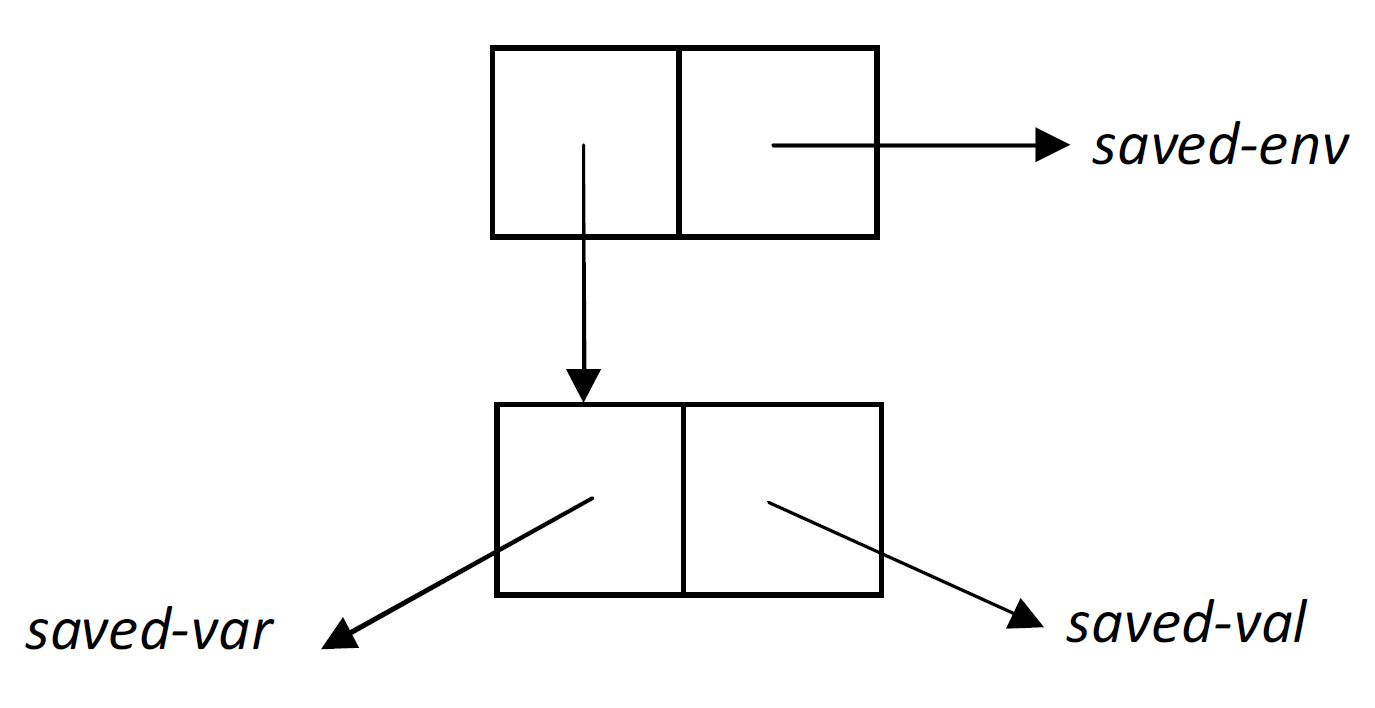
\includegraphics[width=\textwidth]{PS2Q4.PNG}

This is called an \textit{a-list} or \textit{association-list} representation.

\vspace{7.5mm}

\textbf{Problem 5}\footnote{EOPL p.39 Exercise 2.9}: Add to the environment interface (from Problem 4) an observer called \code{has-binding?} that takes an environment \textit{env} and a variable \textit{s} and tests to see if \textit{s} has an associated value in \textit{env}. Implement it using the \textit{a-list} representation.

\end{document}